\section{Question 1}

\begin{question}
    Using the \verb+chredlin+ dataset from the faraway package, do the following:
\end{question}

\subsection{Part a}

\begin{question}
    Define \verb+zips=as.integer(rownames(chredlin))+.
\end{question}

\begin{answer}
    \begin{verbatim}
        library(faraway)
        data(chredlin)
        zips <- as.integer(rownames(chredlin))
    \end{verbatim}
\end{answer}

\subsection{Part b}

\begin{question}
    Make two models in R:
    \begin{align}
        \Omega &: zips \sim theft + fire,\\
        \omega &: zips \sim fire.
    \end{align}
    
\end{question}

\begin{answer}
    I used the following codes to fit the two models:
    \begin{verbatim}
        # Fit two models
        lmO <- lm(zips~theft + fire, data = chredlin)
        lmo <- lm(zips~fire, data = chredlin)
    \end{verbatim}
\end{answer}

\subsection{Part c}

\begin{question}
    Write the two models’ equations. Make sure to keep consistent notation.
\end{question}

\begin{answer}
   The two models' equations are shown below
    \begin{equation}
        \begin{aligned}
            \Omega: zips_{\Omega} & = {{\beta}_{\Omega}}_0 + {{\beta}_{\Omega}}_1 \cdot theft + {{\beta}_{\Omega}}_2 \cdot fire + \epsilon_{\Omega}\\
            \omega: zips_{\omega} & = {{\beta}_{\omega}}_0 + {{\beta}_{\omega}}_2 \cdot fire + \epsilon_{\omega}
        \end{aligned}
    \end{equation}
\end{answer}

\subsection{Part d}

\begin{question}
    Construct $95\%$ confidence level intervals for each of the three parameters in $\Omega$ separately, using matrices. Verify your results using \verb+confint+ in R.
\end{question}

\begin{answer}
    In R, I used the following code to find the $95\%$ confidence level intervals for each parameters in model $\Omega$ by matrices, and I used the R command \verb+confint+ to verify my results.
    \begin{verbatim}
        # Find the degree of freedom
        n <- length(zips)
        p <- 3
        df <- n-p
        # find the critical t-score
        t <- qt(0.975,df)
        t
        # Find the standad errors using matrices
        X <- model.matrix(lmO)
        sigmasq <- t(lmO$fitted-zips)%*%(lmO$fitted-zips)/df
        sigmasq <- sigmasq[1]
        varbetahat <- sigmasq*solve(t(X)%*%X)
        sebetahatcoeff <- (varbetahat^(0.5))[1,1]
        sebetahattheft <- (varbetahat^(0.5))[2,2]
        sebetahatfire <- (varbetahat^(0.5))[3,3]
        # Construct the 95% confidence intervals
        cicoeff <- c(-1,1)*t*sebetahatcoeff + lmO$coeff[1]
        citheft <- c(-1,1)*t*sebetahattheft + lmO$coeff[2]
        cifire <- c(-1,1)*t*sebetahatfire + lmO$coeff[3]
        cicoeff
        citheft
        cifire
        # Verify my results using the confint command in R
        confint(lmO,1,level=0.95)
        confint(lmO,2,level=0.95)
        confint(lmO,3,level=0.95)
    \end{verbatim}
    The $95\%$ confidence interval for the intercept is $(60634.53,60648.93)$. The $95\%$ confidence interval for the parameter of \verb+theft+ is $(-0.36769804,0.04966002)$. The $95\%$ confidence interval for the parameter of \verb+fire+ is $(-0.98757378,0.01253986)$.
    
    The result given by using the command \verb+confint+ is shown in the Figure \ref{fig:fig10}.
     \begin{figure}[H]
        \centering
        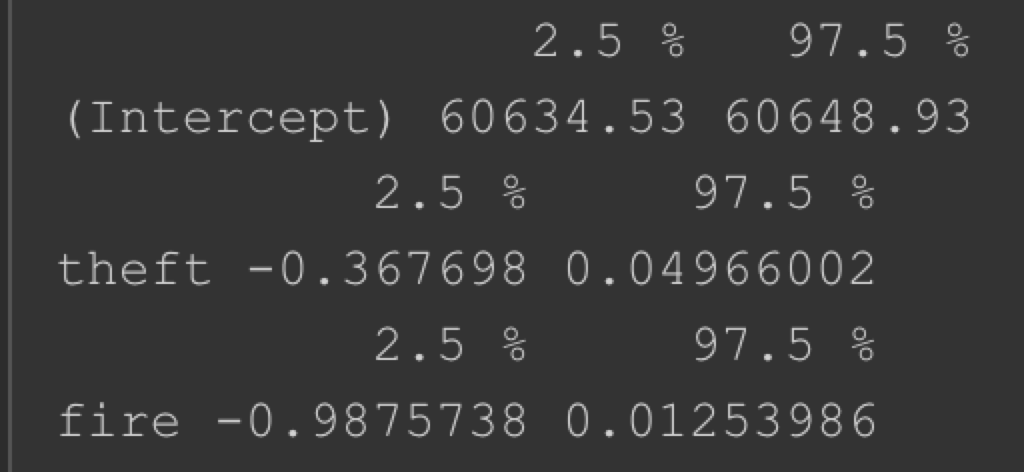
\includegraphics[width=0.5\textwidth]{Figure 10.png}
        \caption{\label{fig:fig10}Results returned by confint in R}
    \end{figure}
    The results are the same.
\end{answer}

\subsection{Part e}

\begin{question}
    Find the $t$-scores for each of the three coefficients in $\Omega$ separately. Find the $p$-values for each of the three coefficients in $\Omega$ separately. Verify your results using \verb+summary+ in R.
\end{question}

\begin{answer}
I used the codes in R to find the t-scores and p values for each parameter, and I compared my results with the results given by R command \verb+summary+.

\begin{verbatim}
    # Find the t-scores for each parameter
    tcoeff <- (lmO$coeff[1] - 0)/sebetahatcoeff
    ttheft <- (lmO$coeff[2] - 0)/sebetahattheft
    tfire <- (lmO$coeff[3] - 0)/sebetahatfire
    tcoeff
    ttheft
    tfire
    # Find the p-values of each parameter
    pvalcoeff <- 2*pt(tcoeff,df)
    pvaltheft <- 2*pt(ttheft,df)
    pvalfire <- 2*pt(tfire,df)
    pvalcoeff
    pvaltheft
    pvalfire
    # Since the pvalcoeff is bigger than 0, we want to use 2(1-pt(t,df)) 
    # to compute its p-value
    pvalcoeff <- 2*(1 - pt(tcoeff,df))
    pvalcoeff
    # Using summary command in R to test my results
    summary(lmO)
\end{verbatim}

The result this gives to me is shown in the Table \ref{tab:tab1}.

\begin{table}[H]
\centering
\caption{Part e results}
\label{tab:tab1}
\begin{tabular}{|c|c|c|}
\hline
\textbf{} & \textbf{t-score} & \textbf{p-value} \\ \hline
$\beta_0$     & 16980.03         & 0                \\ \hline
$\beta_1$     & -1.535764        & 0.1317566        \\ \hline
$\beta_2$     & -1.964828        & 0.05576805       \\ \hline
\end{tabular}
\end{table}

The result given by using the command \verb+summary+ is shown in the Figure \ref{fig:fig11}.
     \begin{figure}[H]
        \centering
        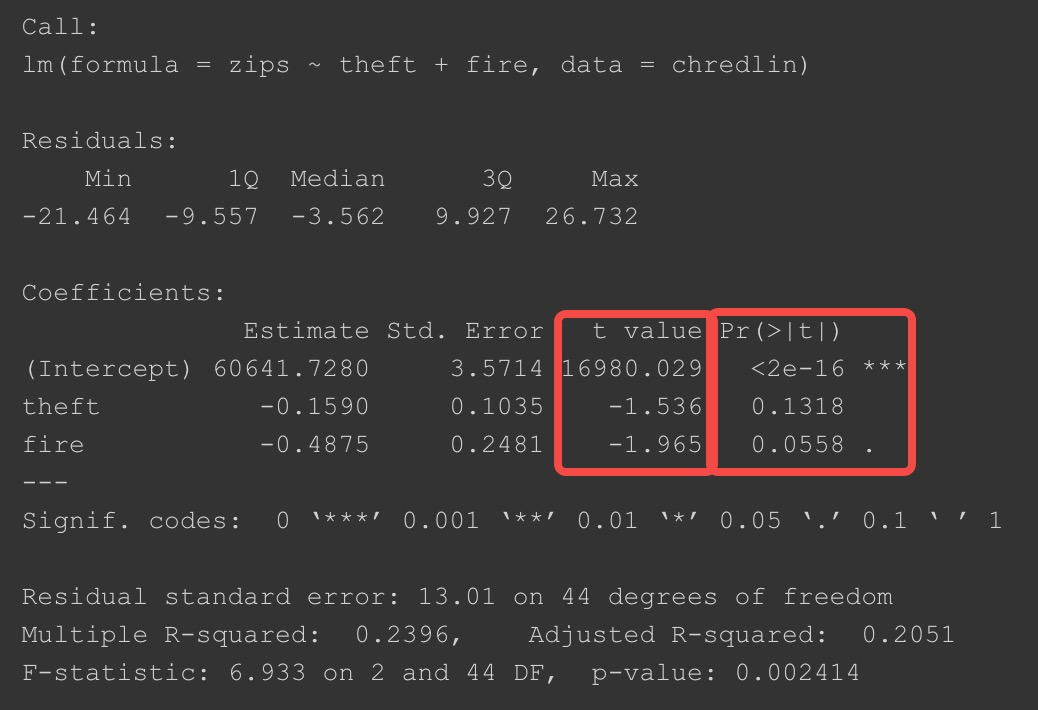
\includegraphics[width=0.7\textwidth]{Figure 11.png}
        \caption{\label{fig:fig11}Results returned by summary in R}
    \end{figure}

I got the same results.
\end{answer}

\subsection{Part f}

\begin{question}
    Test whether each parameter is separately significant to the model at $\alpha = 0.05$.
\end{question}

\begin{answer}
    Since \verb+pvalcoeff+ $\approx 0 < 2*10^{-16} < 0.05$, \verb+pvaltheft+ $= 0.1317566 > 0.05 $ and \verb+pvalfire+ $= 0.05576805 > 0.05$, we reject $H_0$ for $\beta_0$, which is the assumption that $\beta_0 = 0$, but fail to reject $H_0$ for $\beta_1$ and $\beta_2$, which are the assumptions that $\beta_1 = 0$ and $\beta_2 = 0$ separately. Hence, the parameter for the intercept is significant to the model at $\alpha = 0.05$, while the other two parameters are not.
\end{answer}

\subsection{Part g}

\begin{question}
    Determine whether the effect of adding \verb+theft+ to model $\omega$ to make $\Omega$ is statistically significant. Find the $F$ test statistic and $p$-value. How do these compare to (e)?
\end{question}

\begin{answer}
    We start doing this hypothesis testing with hypotheses:
    \begin{align}
        H_0: \omega &: zips \sim fire \text{ is better.}\\
        H_A: \Omega &: zips \sim theft + fire \text{ is better.}
    \end{align}
    Then, I used the following code to find the F-statistic and p-value for this hypothesis test.
    \begin{verbatim}
        # Find SSE for both models
        SSEO <- (t(lmO$residuals)%*%lmO$residuals)[1]
        SSEo <- (t(lmo$residuals)%*%lmo$residuals)[1]
        q <- dim(model.matrix(lmo))[2]
        # Find the F-statistic
        Fstat <- ((SSEo-SSEO)/(p-q))/(SSEO/(n-p))
        Fstat
        # Find the p-value
        pvalF <- 1-pf(Fstat,p-q,n-p)
        pvalF
        # Find the Fstar
        Fstar <- qf(0.95,p-q,n-p)
        Fstar
    \end{verbatim}
    R returns us  the result that $F = 2.358571 < 4.061706 = F^{*}$, and $p-value = 0.1317566 > 0.05$, so this shows to us that we fail to reject $H_0$. In the other word, we accept $H_0$. Hence adding \verb+theft+ to model $\omega$ to make is not statistically significant at $\alpha = 0.05$. Comparing to Part e, the p-value here is the same as the p-value for \verb+theft+, and the F-statistic is the square of the t-score of $\beta_1$, which makes sense, since the model $\Omega$ is different from the model $\omega$ at the point that it add a new variable \verb+theft+.
    \end{answer}

\subsection{Part h}

\begin{question}
    Test whether the combined effect of \verb+fire+ and \verb+theft+ is statistically significant to $\Omega$.
\end{question}

\begin{answer}
     We could test the combined effect of \verb+fire+ and \verb+theft+ with hypotheses:
    \begin{align}
        H_0: \omega_0 &: zips \sim 1 \text{ is better.}\\
        H_A: \Omega &: zips \sim theft + fire \text{ is better.}
    \end{align}
    Then, I used the following code to find the F-statistic and p-value for this hypothesis test.
    \begin{verbatim}
       # Fit the trival model omega0
        lmo0 <- lm(zips~1)
        # Find the SSE for this model
        SSEo0 <- (t(lmo0$residuals)%*%lmo0$residuals)[1]
        q0 <- dim(model.matrix(lmo0))[2]
        # Find the F-statistic
        Fstat0 <- ((SSEo0-SSEO)/(p-q0))/(SSEO/(n-p))
        Fstat0
        # Find the p-value
        pvalF0 <- 1-pf(Fstat0,p-q0,n-p)
        pvalF0
        # Find the Fstar
        Fstar0 <- qf(0.95,p-q0,n-p)
        Fstar0
    \end{verbatim}
    R returns us  the result that $F = 6.932705 > 3.209278 = F^{*}$, and $p-value = 0.002414016 < 0.05$, so this shows to us that we reject $H_0$. In the other word, we accept $H_A$. Hence, \verb+fire+ and \verb+theft+ have a statisticall significant combined effect to $\Omega$.
\end{answer}

\subsection{Part i}

\begin{question}
    Why might rates of fires and thefts be related to zip code as a number (not a category)?
\end{question}
   
\begin{answer}
    This might be because that the zip codes are not showing locations that are totally unrelated. Locations with closed zip codes are normally neighbours of each other. Thus, fires and thefts often happen in the near neighbourhoods. 
\end{answer}

\subsection{Part j}

\begin{question}
    Plot $95\%$ confidence intervals for each of the two parameters in $\omega$ to make a rectangle.
\end{question}

\begin{answer}
I draw the triangle using the code below and get a result in Figure \ref{fig:fig12}.
    \begin{verbatim}
        # First plot the estimate
        plot(lmo$coeff[1],lmo$coeff[2], xlab = "intercept",
        ylab = "beta_fire", xlim=c(60630,60650), ylim=c(-2,0))
        # Construct the rectangle
        vlow <- confint(lmo)[1]
        vhigh <- confint(lmo)[3]
        hlow <- confint(lmo)[2]
        hhigh <- confint(lmo)[4]
        # Draw the lines
        abline(v = vhigh,col = 'red')
        abline(v = vlow,col = 'red')
        abline(hlow,0, col = 'steelblue')
        abline(hhigh,0, col = 'steelblue')
    \end{verbatim}
    \begin{figure}[H]
        \centering
        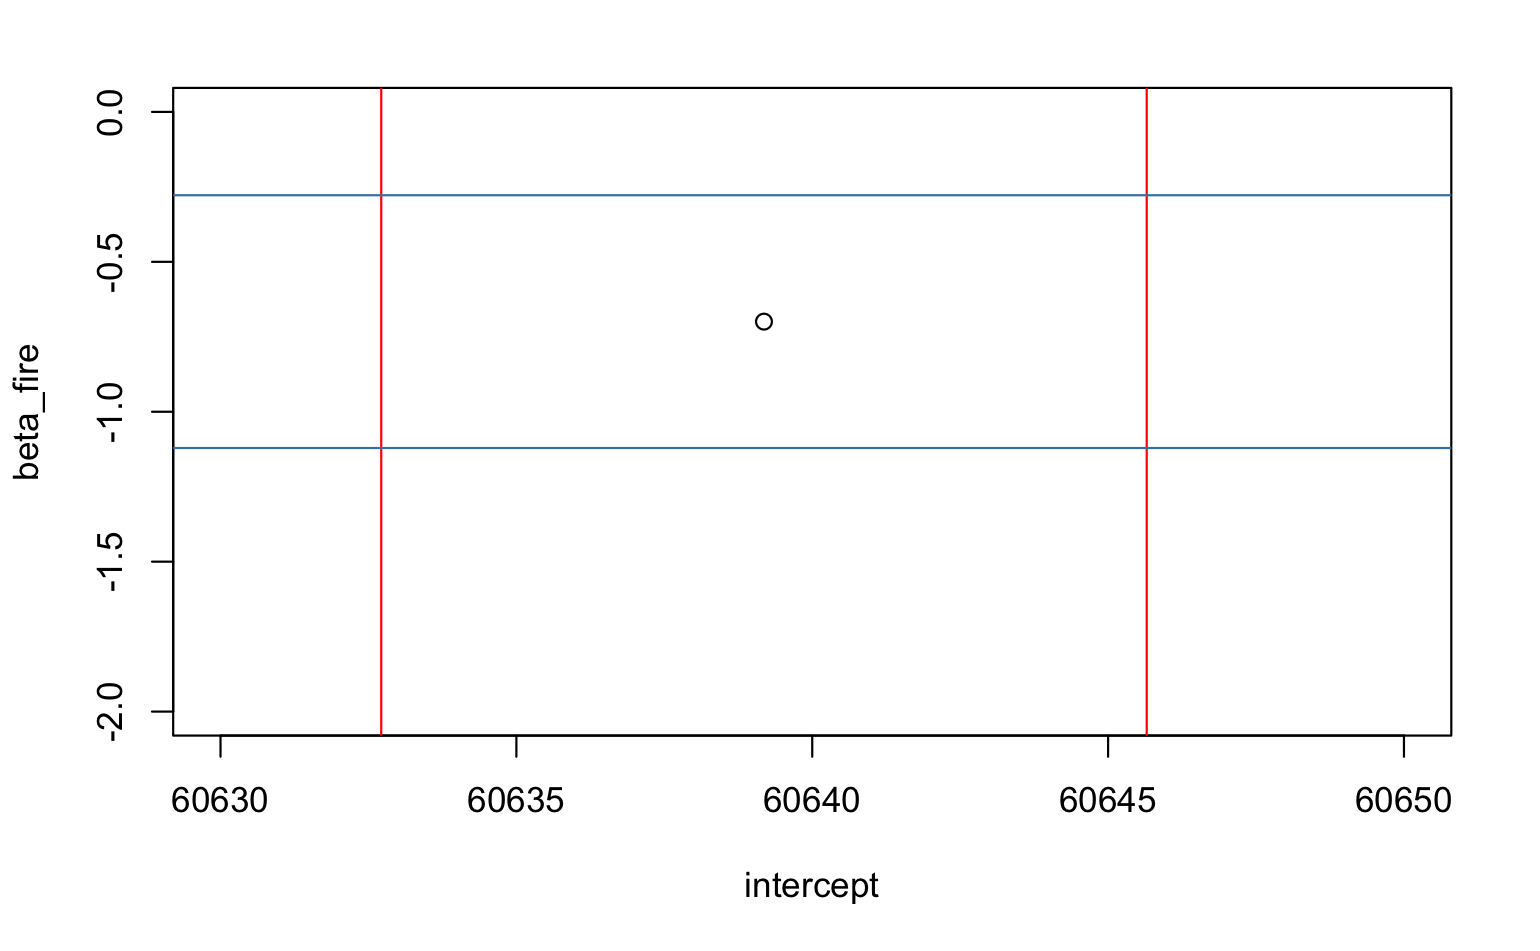
\includegraphics[width=0.7\textwidth]{Figure 12.png}
        \caption{\label{fig:fig12}95\% confidence intervals for two parameters in omega in rectangle form}
    \end{figure}
\end{answer}

\subsection{Part k}

\begin{question}
    Plot a $95\%$ confidence region for the two parameters in $\omega$ together over the same graph.
\end{question}

\begin{answer}
    I used the code below to plot a $95\%$ confidence region for the two parameters in $\omega$ together over the same graph in part j and got a result in Figure \ref{fig:fig13}.
    \begin{verbatim}
        # Install the package "ellipse"
        # (Uncomment the next line if it is not installed before)
        #install.packages("ellipse")
        library(ellipse)
        ellipse(lmo)
        # plot the $95\%$ confidence region
        plot(ellipse(lmo),type = "l",xlim=c(60630,60650), ylim=c(-2,0))
        points(lmo$coeff[1],lmo$coeff[2])
        vlow <- confint(lmo)[1]
        vhigh <- confint(lmo)[3]
        hlow <- confint(lmo)[2]
        hhigh <- confint(lmo)[4]
        # Draw the lines
        abline(v = vhigh,col = 'red')
        abline(v = vlow,col = 'red')
        abline(hlow,0, col = 'steelblue')
        abline(hhigh,0, col = 'steelblue')
    \end{verbatim}
    \begin{figure}[H]
        \centering
        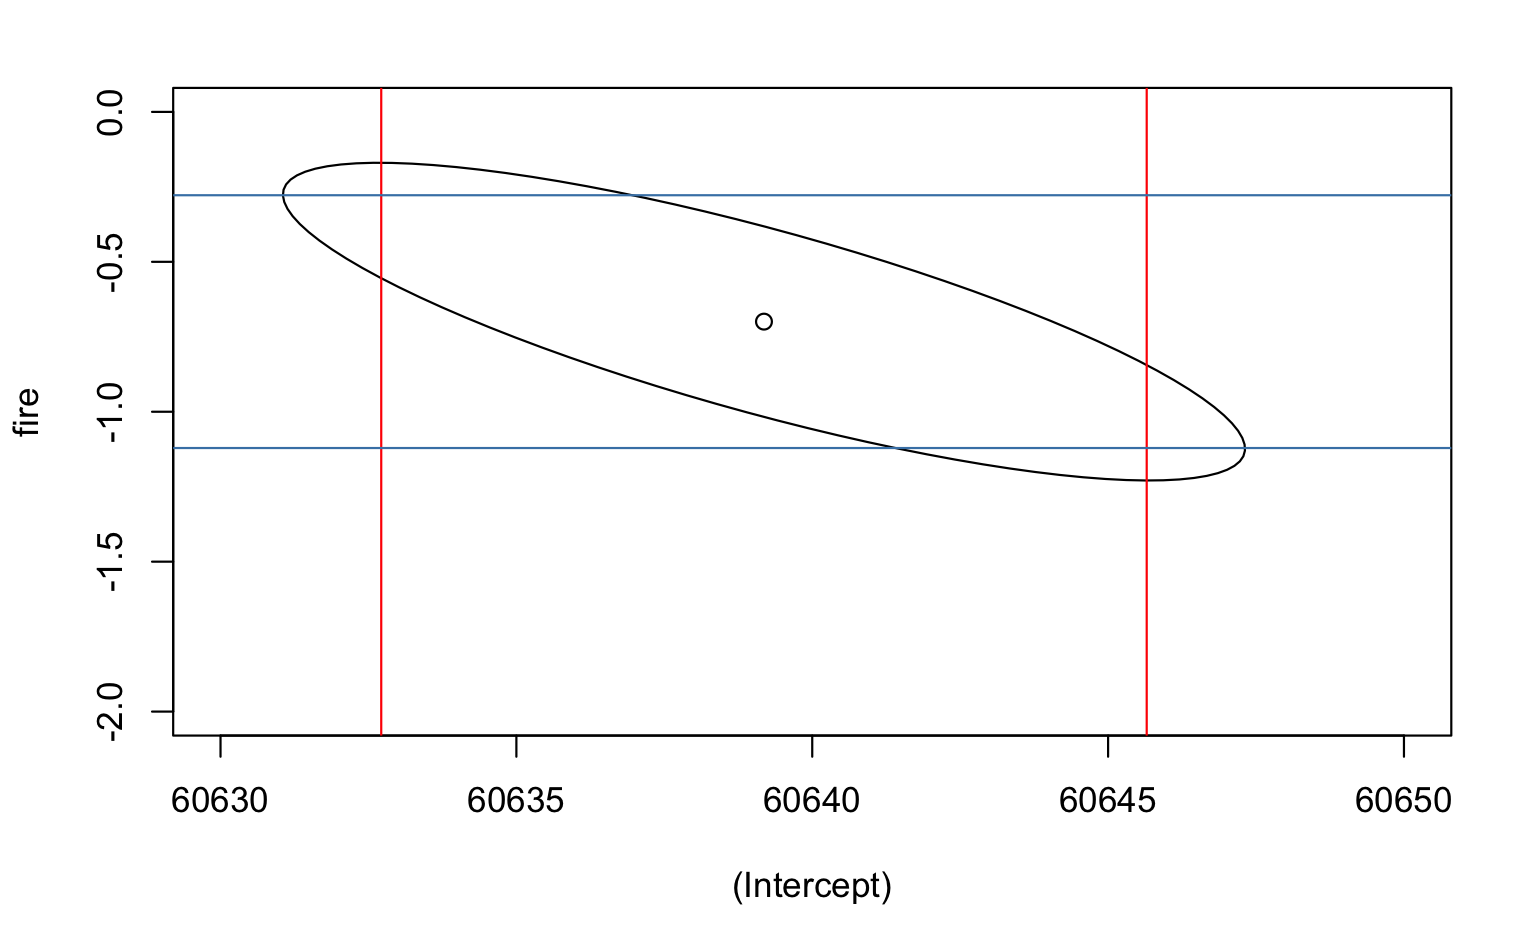
\includegraphics[width=0.7\textwidth]{Figure 13.png}
        \caption{\label{fig:fig13}95\% confidence region for two parameters in omega}
    \end{figure}
\end{answer}